\documentclass[conference]{IEEEtran}
\IEEEoverridecommandlockouts
\usepackage{cite}
\usepackage{amsmath,amssymb,amsfonts}
\usepackage{algorithmic}
\usepackage{graphicx}
\usepackage{textcomp}
\usepackage{xcolor}
\def\BibTeX{{\rm B\kern-.05em{\sc i\kern-.025em b}\kern-.08em
    T\kern-.1667em\lower.7ex\hbox{E}\kern-.125emX}}
\begin{document}

\title{An Integrated Multi-Task Machine Learning Workflow for Data-driven Therapeutic Development: From Molecular Screening to Clinical Outcome Prediction\\
}

\author{\IEEEauthorblockN{Swetha Balasubramanian}
\IEEEauthorblockA{\textit{MSc. Data Science} \\
\textit{University of Bristol}\\
Bristol, United Kingdom \\
swethabala042@gmail.com}
}
\maketitle

\begin{abstract}
In today’s rapidly evolving world, the healthcare sector has become the essential foundation for all other fields, and drug discovery, in turn, forms the central pillar of healthcare;Nevertheless, it remains the most intricate undertaking, requiring a process of 10–15 years, encompassing multiple stages and costs that exceed \$2 billion per approved therapy. Although volumes of biological, chemical, and clinical data are increasing, current therapeutic pipelines are fragmented and employ uncoordinated workflows that are slow to incorporate new evidence and prone to costly late-stage failure. The majority of existing machine learning techniques used in drug development have been applied to isolated sub tasks rather than being combined into coherent decision support frameworks. The project presented here aims to design a comprehensive data-driven workflow that integrates heterogeneous data sources through the various stages of the therapeutic pipeline. This approach incorporates multi-task deep learning with interpretable feature selection methods and strong cross-validation approaches to enable increased prediction accuracy and generalization to novel classes of compounds. By modeling the therapeutic development pipeline as a chained set of data transformations, as opposed to isolated prediction problems, it is anticipated that attrition rates and development cycles may be decreased while actionable information can be generated at each step in the pipeline. 
\end{abstract}

\begin{IEEEkeywords}
drug discovery, therapeutic development, machine learning
pipeline, ADMET prediction, multi-task learning, data
integration
\end{IEEEkeywords}

\section{Introduction}
The development of a new therapeutic agent is one of the most expensive and failure-prone processes in modern science. Fewer than 10 \% of the candidates who enter the Phase I trials ultimately receive approval \cite{b1}. On average, the cost of bringing an approved drug to market exceeds \$2 billion when estimating the cost of failures \cite{b2}. Failure in Phase II or III clinical trials can result in losses ranging from \$800 million to \$1.4 billion, encompassing not only trial expenses but also all previous preclinical work \cite{b1}. Socially, this prolongs the wait for new drugs and discourages the investigation of promising biological hypotheses due to logistical challenges rather than scientific invalidity. In fact, more than 80\% of drug failures are attributed to suboptimal ADMET properties, suggesting that increasing the use of computational models early in the development pipeline could significantly reduce this waste \cite{b8}.

Much of this attrition can be attributed to the largely disconnected modular nature of current drug discovery pipelines. Data generated at various stages of the process-from molecular screening, toxicity studies and biomarker identification, to the ultimate outcome of the clinical trial-are generally not integrated \cite{b3}. Each stage's machine learning models at each stage address isolated sub-problems. Consequently, important informational relationships across the pipeline are lost at every stage of the transition, weakening the overall predictive power. Furthermore, the gap between benchmark performance and real-world outcomes has largely gone unaddressed.

The cost of failing to address this problem is both demonstrable and significant. Each year that the pipeline remains inefficient results in delays in life-saving treatments, wastes billions on failed leads, and erodes public confidence in computational methods that, with proper integration and validation, could fundamentally transform drug discovery. Stokes et al. \cite{b11} demonstrated this potential with a single graph neural network that screened 107 million compounds in four days to identify a new antibiotic, Halicin; however, this approach addresses only the identification of leads. A fully machine-driven solution encompassing the entire pipeline has yet to be realized.

\section{Critical Literature Review}
Machine learning in drug discovery is over 20 years old and has progressed from QSAR with fixed molecular descriptors, through ensemble classifiers, to deep graph-based models, and multi-modal integration frameworks. A five-year narrative review shows that the process has evolved from empirical screening to data-driven design; however, it points out that benchmark performance is almost always inflated compared to real-world data and clinical validation of AI discovered drugs have not yet appeared \cite{b2}. The paper providing the most complete pipeline covering review \cite{b3} places ``data integration across pipeline stages" at its center, a diagnosis that remains relevant six years later. The paper reviews 5 methodological clusters, takes 5 founding papers that can be broken down deeply using the `CRAAP' framework, and reconciles contradictions to establish the proposed research gap.

\subsection{Classic Machine Learning}
Early workflows used fixed molecular descriptors in support vector machine and random forest models, proving the viability of computation screening but being hampered by two structural failings; (i) fixed fingerprints are unsuited to prediction tasks, and (ii) models trained in chemical series overgeneralize structures outside of this series, \cite{b3}. The MoleculeNet benchmark \cite{b6}, (CRAAP score:22/25), a field benchmark, used 17 datasets comprising 700,000 molecules to show that learnable graph representations outperform fixed descriptors. MoleculeNet suffers from both duplicate molecules between training and testing, and random splitting, which will lead to data leakage, \cite{b4}. So, while there is evidence that GNNs perform better than fixed descriptors, it cannot be relied upon due to data leakage until reproduced by scaffold split validation, a discovery upon which many further steps were relied.

\subsection{Deep Learning for Molecular Property Prediction}
 Yang et al. \cite{b5} built a directed message passing neural network (D-MPNN) in which the passing of messages over directed bonds occurs exactly once; thus without redundancy, this is chosen as the foundation source for methodological rigour and immediate relation to the structure of this portfolio (CRAAP score: 24/25). D-MPNN in 19 public and 16 industrial proprietary datasets yielded far superior results compared to MoleculeNet benchmarks. In particular, Yang et al. \cite{b5} showed how scaffold-based splits yield far more conservative but more realistic performance estimates compared to random splits, suggesting that this is the new standard. The literature has largely disregarded this advice \cite{b4}.
 
 The key demonstration is Stokes et al. \cite{b11}, is chosen as the foundation source for the strongest empirical evidence of data-driven therapeutic discovery (CRAAP Score: 23/25). A GNN trained in 2,560 compounds screened 107 million to identify halicin. Bacteria did not develop resistance over 30 days, while they developed resistance over 1 –3 days for ciprofloxacin. However, the evidence reveals that the workflow covered only the identification of skewness: ADMET profile, toxicity assessment, and clinical outcome modeling were completely absent, and halicin has not entered human clinical trials. The claim that a complete data-driven therapeutic workflow is achievable is not supported by the authors' own evidence -- this paper demonstrates one stage, not the pipeline.

\subsection{ADMET Prediction Workflows}
The evaluation of ADMET is the single most problematic pipeline bottleneck (more than 80\% of drug failure is due to poor properties of ADMET) \cite{b8}, and attrition has moved from pharmacokinetic failure to preclinical toxicology and clinical tolerability. Shaker et al. \cite{b7}, which is used as a source since it is the latest available review(CRAAP Score: 22/25), notes that the current methods use GNNs. Shaker et al. \cite{b7} clearly name the single-modal data reliance and model opacity as the two main problems that still need to be solved. Each platform they looked at works on its own, ignoring the informational dependencies between ADMET endpoints and downstream stages that multi-stage integration would keep.

\subsection{End-to-end pipeline}
Vamathevan et al \cite{b3} is chosen as the `core' paper, because of the only available in-depth pipeline analysis (CRAAP Score: 22/25) and identifies the absence of standardized data connecting pipeline stages as a bottleneck for integration. By July 2025, there were 29+ AI driven programs in human trials \cite{b2}. Rentosertib was one example of a drug and had positive Phase IIa results by 2025, being the first to reach the stage of demonstrating both safety and efficacy in a human trial \cite{b2}. In contrast, DSP-1181 was discontinued after Phase I, suggesting that speed is not directly proportional to clinical effectiveness. Additionally, Bender and Cort\'{e}s-Ciriano \cite{b9} criticize the use of biological training from animal or cell line biological training data as systematically biased proxies for human clinical outcomes and suggest that they could make technically advanced pipelines unreliable.

\subsection{Ethics and Validity Issues }
Bender and Cort\'{e}s-Ciriano \cite{b4} -- chosen as a foundational resource for the most authoritative criticism of validation practices across the field (CRAAP Score: 22/25) -- list three common problems: random splitting, data leakage, and absence of external replication. Harrer et al. \cite{b1} noted that AI-based cohort selection runs the risk of propagating biases within EHRs among demographics. Obermeyer et al. \cite{b10} offers the most concrete example of a clinical consequence from a trained model's bias: a commercial healthcare algorithm influencing 200 million patients was found to consistently under-refer Black patients to specialty care, substituting hospital charges for healthcare need, which dropped black patients' access to specialist care from 46.5 to 17.7\%. When re-designed to optimize directly for health instead of cost, this reduced the racial gap in referrals by 84\%; the gap was clearly both required and resolvable.

\subsection{Synthesis}
A consistent structural limitation emerges across all five Methodological clusters: the therapeutic pipeline is treated as a sequence of independent prediction problems rather than a connected system. Classic ML generalizes poorly beyond training chemistry. Deep learning models overestimate out-of-distribution performance due to evaluation protocol failures \cite{b4, b5}. The ADMET tools are mature but siloed, discarding inter-stage dependencies \cite{b7, b8}. End-to-end pipelines cover at most two stages and carry limited clinical validation \cite{b3, b2}. Ethical vulnerabilities are identified but treated as peripheral rather than as design requirements \cite{b10, b9}. The field has clearly diagnosed what is wrong; no published framework has addressed these limitations in combination.

 
\section{Research Gap and Objectives}
Currently, no published framework currently simultaneously combines molecular property prediction, ADMET profiling, and clinical outcome modeling at several stages of therapeutic development while also guaranteeing out-of-distribution generalization using a scaffold-based approach \cite{b5}, managing missing modalities across heterogeneous sources, providing adequate interpret-ability for expert-level decision making \cite{b7}, and instilling bias-reduction as a first-class design consideration \cite{b10}. All of these four requirements individually have been shown in previous work to be needed and have not, prior to this, been put together in a single, confirmed, and tested system.

\subsection{Research Question}
How does a multi-task, multi-modal machine learning workflow - incorporating molecular fingerprint data, bio activity measurements, and clinical outcome data - fare in improving drug candidate attrition predictions over the course of early drug development compared to single task and single modality baseline models, evaluated on out-of-distribution conditions in a scaffold-split manner?

\subsection{SMART Objectives}
 
\begin{enumerate}
 
\item \textbf{Objective 1 : Dataset} The proposed workflow must prove it can fuse heterogeneous data sources from across multiple pipeline stages into a single, ready-to-use input. Procure and pre-process ChEMBL~v33 bio-activity measurements, DrugBank drug-target interaction annotations, and transcriptomic perturbation signatures; perform confidence score filtering; convert activity measurements to a pIC50 scale; normalize molecular identifiers to the InChIKey standard; calculate and document missing value percentages; determine license status of each source. The goal is a unified analysis ready dataset with provenance information ready to be used directly by the model at the end of week 3.
 
\item \textbf{Objective 2 : Pipeline and Model Design} To suggest a feasible system, a complete specification of a pipeline that could technically be built, measured, and compared with other benchmarks is needed. Design and implement a 5 stage data-driven pipeline and a D-MPNN multi-task neural network that predicts minimum of 5 ADMET endpoint activities and bioactivity labels, justifying each design decision with at least one citation from literature; identify and justify two models for baseline comparison (random forest on Morgan fingerprints and single task D-MPNN) under identical scaffold split evaluation conditions. The goal is to complete a pipeline specification and architecture diagram with citation-backed justifications for each methodological choice by the end of Week~6.
 
\item \textbf{Objective 3 --- Validation and Ethics}  In order to answer the research question, evaluation method that fairly assess generalization performance on new compounds and does not simply report an inflated benchmark, as found by Bender and Cort\'{e}s-Ciriano~\cite{b4}, should be defined. This objective provides the initial steps in identifying the ethical implications of a skewed training set \cite{b10}: defines scaffold based training and test sets \cite{b5} to ensure novel chemical scaffolds are predicted on the test set; selected relevant primary (AUC-ROC, precision-recall AUC, RMSE) and secondary (BEDROC) metrics for imbalanced end points; conducted an ethical risk audit identifying 3 classes of risk (class imbalance, coverage bias, model opacity) with at least one associated concrete, technical mitigating factor. The goal is Final validation protocol and ethical risk assessment document completed by end of Week 9, and with one citation to each ethical risk's mitigating factor.

\end{enumerate}

\section{Proposed Methodology} 
\subsection{Technical Pipeline}
The proposed workflow involves five comprehensive
steps. \textit{(1) Data extraction:} Compound records, bioactivity measurements, and transcriptomic perturbation data should be extracted  from ChEMBL, DrugBank, and LINCS L1000 databases. Molecular features should be normalized to the common molecular identifiers of the compound using InChIKey, while the assay records were filtered according to the given assay confidence score.\textit{(2) Molecular Graph:} molecules should be converted into directed molecular graphs which serves as the input feature for D-MPNN, and also converted to Morgan fingerprint vector for baseline comparisons. \textit{(3) Multi-task model training:} a shared D-MPNN encoder should be trained to generate the molecular representations. Task specific prediction heads should be connected to this encoder which in turn predicts ADMET endpoints and bioactivity label simultaneously, thus maintaining the relationship between the two predictions. \textit{(4) Out-of-distribution validation:} models should be evaluated in scaffold-split hold-out sets that only contain chemical scaffolds not seen in the training set\cite{b5}. \textit{(5) Interpretability analysis:} The SHAP value should be calculated for each prediction to obtain the features of the molecules that influence each prediction, thus providing an interpretability layer that experts can interpret\cite{b7}.Each stage is directly linked to the subsequent stage, and therefore no information flow between stages was discarded as in silos approaches\cite{b3}.
 
\subsection{Justification}
The D-MPNN method is chosen over fixed fingerprint methods because Yang et al. \cite{b5} demonstrated superior performance on realistic scaffold-split evaluations in public and private datasets, and the success in the large-scale identification of novel chemical candidates from Stokes et al. \cite{b11}. Multi-task learning is chosen, due to the successful results in the prediction of multiple ADMET properties simultaneously over individual properties by Shaker et al. \cite{b7}. Scaffold-based splitting is chosen to directly address data leakage as identified by Bender and Cort\'{e}s-Ciriano \cite{b4}.
 
\subsection{Baseline and Evaluation Metrics}
 
The two baselines that will be evaluated are: (1) a random forest on Morgan fingerprints, representing the state of the art prior to deep learning methods \cite{b3}, and (2) a series of single-task D-MPNN models, one for each endpoint (so as to separate the multi-task effect from the graph representation). The evaluation metrics to be used are AUC-ROC and precision-recall AUC for classification tasks and RMSE for regression tasks. In case of severe class imbalance, the metric BEDROC, will supplement AUC-ROC as a ranking-sensitive metric appropriate for virtual screening.

\section{Data, Ethics, and Practical Considerations} 
\subsection{Data Readiness}
 
\textbf{ChEMBL v33} (CC BY-SA 3.0) consists of more than 2 million compounds with bioactivity information. Diverse conditions will be standardized to the pIC50 values, with confidence score filtering ($\geq$8) to exclude unreliable entries. \textbf{DrugBank} contains validated ADMET information, but is biased towards the well-characterized and approved drugs, making it poor for less-explored target spaces and diseases. \textbf{LINCS L1000} (NIH public access) contains transcriptomic perturbation signatures for roughly 30,000 compounds. However,its limitation is its use of 978 landmark genes means that a large amount of the genome's transcriptome is discarded.
 
\subsection{Ethical Red-Teaming}
 
Risks are classified into three main categories by failure analysis, each with a corresponding mitigation strategy. \textbf{Class imbalance:} negative examples (failed candidates) are under-represented due to publication bias, which can lead to models that systematically favour predicted success and fail to flag problematic candidates. \textbf{Coverage bias:} target families, such as kinases and GPCRs, and compound chemical space based on Western laboratory cultures are highly over-represented in many available databases \cite{b10}. This results in poor performance on diseases that are not widely studied, as well as non-European metabolic disease profiling. \textbf{Model opacity:} the predictions made by the multi-task D-MPNN are not directly explainable, risking misuse by users who are not experts. 

\subsection{Mitigation}
Class imbalance can be mitigated by using cost-sensitive cross-entropy loss functions; and using SMOTE oversampling prior to model training. Coverage bias can be mitigated by stratified sampling of training data according to target family; evaluation of performance over different target subgroups; flagging of predictions made on compounds that are sufficiently distant from the training set distribution. Model opacity can be mitigated by the generation of SHAP values for individual predictions, which give a measure of the importance of each molecular characteristic in the final prediction, allowing domain experts to investigate whether a given prediction is driven by reasonable chemical motifs \cite{b7}.

\section{Project Planning}
The project is designed to have a 12-week lifecycle, with 4 consecutive phases, each with defined milestone dependencies:
\begin{enumerate}
\item \textit{(Weeks 1-3): Literature Survey}: Read and annotate all foundation papers. \item \textit{(Week 4) Dataset}: Obtain and preprocess the three datasets.\item \textit{(Weeks 5-6): Methodology Design-} Write pipeline and select architecture of the D-MPNN and set up the baselines.\item \textit{(Weeks 7-8): Validation and Ethics}: Create the scaffold-based framework and document the bias audit and the proposed mitigating strategies.\item \textit{(Weeks 9-12): Documentation}: Complete the entire IEEE draft.
\end{enumerate}
The Gantt chart is as follows: 
\begin{figure}[h]
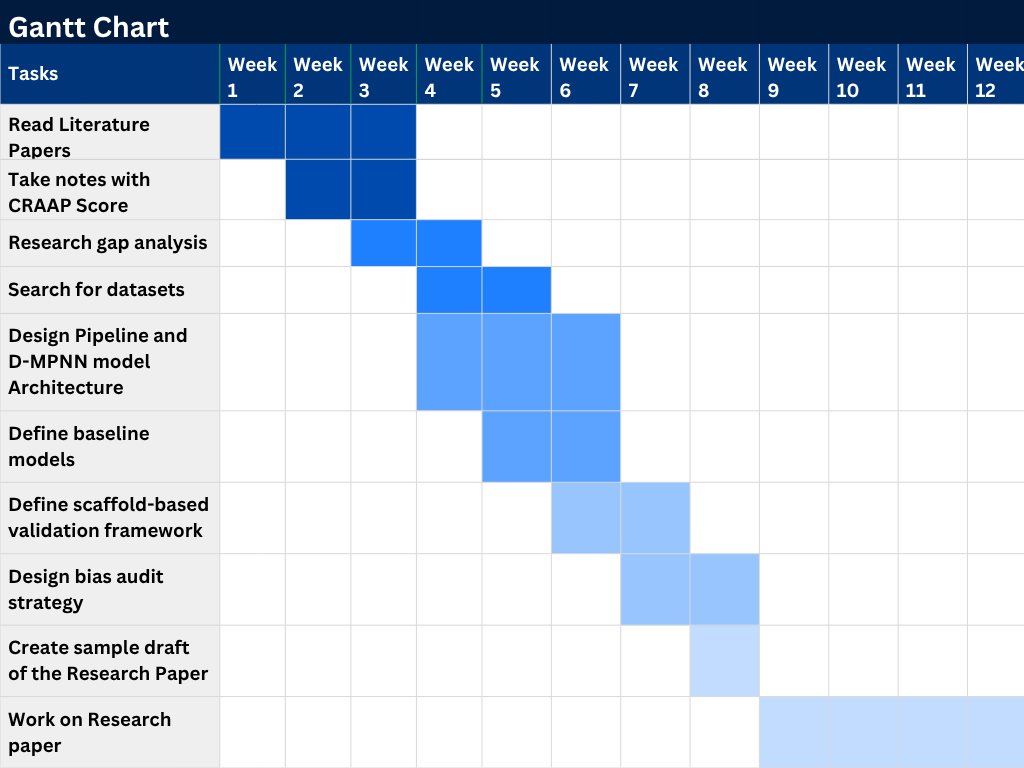
\includegraphics[width=9cm]{Task Names.png}
\caption{Gantt Chart}
\end{figure}
The trello link for the project management board is: \texttt{https://trello.com/b/qtWvkiVn/portfolio}.

\section{Non-Technical Summary}
Drug discovery, the process of developing new drugs, is very complex, taking about a decade; is very expensive; and consists of complex processes. Every drug that reaches the patient there are hundreds which have failed, after years of work and spending huge amounts of money,


\begin{thebibliography}{00}
\bibitem{b1} Stefan Harrer, Pratik Shah, Bhavna Antony, and Jianying Hu, ``Artificial Intelligence for Clinical Trial Design,'' in Trends in Pharmacological Sciences, 2019.
\bibitem{b2} Vikrant Verma, and Dharmendra Kumar, ``Artificial intelligence and machine learning in drug discovery: From lead discovery to clinical validation (2020–2025),'' in Life Sciences, 2026.
\bibitem{b3} Jessica Vamathevan, Dominic Clark, Paul Czodrowski, Ian Dunham,Edgardo Ferran, George Lee, Bin Li, Anant Madabhushi, Parantu Shah,
Michaela Spitzer and Shanrong Zhao, ``Applications of machine learning in drug discovery and development,'' in Nature Reviews Drug Discovery, 2019.
\bibitem{b4} Claudio N. Cavasotto, Juan I. Di Filippo and Valeria Scardino, ``Lessons learnt from machine learning in early stages of drug discovery,'' in Expert Opinion on Drug Discovery, 2024.
\bibitem{b5} Kevin Yang, Kyle Swanson, Wengong Jin, Connor Coley, Philipp Eiden, Hua Gao, Angel Guzman-Perez, Timothy Hopper, Brian Kelley, Miriam Mathea, Andrew Palmer, Volker Settels, Tommi Jaakkola, Klavs Jensen, and Regina Barzilay, ``Analyzing Learned Molecular Representations for Property
Prediction,'' in Journal of Chemical Information and Modeling, 2019.
\bibitem{b6} Zhenqin Wu, Bharath Ramsundar, Evan N. Feinberg, Joseph Gomes, Caleb Geniesse, Aneesh S. Pappu, Karl Leswing, and Vijay Pande, ``MoleculeNet: A Benchmark for Molecular Machine Learning,'' in Chemical Science, 2019.
\bibitem{b7} Nini Fan, Jing Chen, Jinghui Wang, Zhe-Cheng Chen, Yinfeng Yang, ``Bridging data and drug development: Machine learning approaches for next-generation ADMET prediction,`` in Drug Discovery Today, November 2025.
\bibitem{b8} Magesh Venkataraman, Gopi Chand Rao, Jeevan Karthik Madavareddi and Srinivas Rao Maddi, ``Leveraging machine learning models in evaluating ADMET properties for drug discovery and development,`` in ADMET and DMPK, June 2025.
\bibitem{b9} Andreas Bender and Isidro Cortes-Ciriano, ``Artificial intelligence in drug discovery: what is realistic, what are illusions? Part 2: a discussion of chemical and biological data,`` in Drug Discovery Today, April 2021.
\bibitem{b10} Ziad Obermeyer, Brian Power, Christine Vogeli, Sendhil Mullainathan, ``Dissecting racial bias in an algorithm used to manage
the health of populations ,`` in Science, 2021.
\bibitem{b11} Jonathan M. Stokes, Kevin Yang, Kyle Swanson, ..., Tommi S. Jaakkola, Regina Barzilay, James J. Collins, ``A Deep Learning Approach to Antibiotic Discovery,`` in Cell, February 2020.
\end{thebibliography}
\end{document}
